%% abtex2-modelo-artigo.tex, v<VERSION> laurocesar
%% Copyright 2012-<COPYRIGHT_YEAR> by abnTeX2 group at http://www.abntex.net.br/ 
%%
%% This work may be distributed and/or modified under the
%% conditions of the LaTeX Project Public License, either version 1.3
%% of this license or (at your option) any later version.
%% The latest version of this license is in
%%   http://www.latex-project.org/lppl.txt
%% and version 1.3 or later is part of all distributions of LaTeX
%% version 2005/12/01 or later.
%%
%% This work has the LPPL maintenance status `maintained'.
%% 
%% The Current Maintainer of this work is the abnTeX2 team, led
%% by Lauro César Araujo. Further information are available on 
%% http://www.abntex.net.br/
%%
%% This work consists of the files abntex2-modelo-artigo.tex and
%% abntex2-modelo-references.bib
%%

% ------------------------------------------------------------------------
% ------------------------------------------------------------------------
% abnTeX2: Modelo de Artigo Acadêmico em conformidade com
% ABNT NBR 6022:2018: Informação e documentação - Artigo em publicação 
% periódica científica - Apresentação
% ------------------------------------------------------------------------
% ------------------------------------------------------------------------

\documentclass[
	% -- opções da classe memoir --
	article,			% indica que é um artigo acadêmico
	12pt,				% tamanho da fonte
	oneside,			% para impressão apenas no recto. Oposto a twoside
	a4paper,			% tamanho do papel. 
	% -- opções da classe abntex2 --
	%chapter=TITLE,		% títulos de capítulos convertidos em letras maiúsculas
	%section=TITLE,		% títulos de seções convertidos em letras maiúsculas
	%subsection=TITLE,	% títulos de subseções convertidos em letras maiúsculas
	%subsubsection=TITLE % títulos de subsubseções convertidos em letras maiúsculas
	% -- opções do pacote babel --
	english,			% idioma adicional para hifenização
	brazil,				% o último idioma é o principal do documento
	sumario=tradicional
]{abntex2}


% ---
% PACOTES
% ---

% ---
% Pacotes fundamentais 
% ---
\usepackage{lmodern}			% Usa a fonte Latin Modern
\usepackage[T1]{fontenc}		% Selecao de codigos de fonte.
\usepackage[utf8]{inputenc}		% Codificacao do documento (conversão automática dos acentos)
\usepackage{indentfirst}		% Indenta o primeiro parágrafo de cada seção.
\usepackage{nomencl} 			% Lista de simbolos
\usepackage{color}				% Controle das cores
\usepackage{graphicx}			% Inclusão de gráficos
\usepackage{microtype} 			% para melhorias de justificação
\usepackage{multirow}
\usepackage{float}
% ---
		
% ---
% Pacotes adicionais, usados apenas no âmbito do Modelo Canônico do abnteX2
% ---
\usepackage{lipsum}				% para geração de dummy text
% ---
		
% ---
% Pacotes de citações
% ---
\usepackage[brazilian,hyperpageref]{backref}	 % Paginas com as citações na bibl
\usepackage[alf]{abntex2cite}	% Citações padrão ABNT
% ---

% ---
% Configurações do pacote backref
% Usado sem a opção hyperpageref de backref
\renewcommand{\backrefpagesname}{Citado na(s) página(s):~}
% Texto padrão antes do número das páginas
\renewcommand{\backref}{}
% Define os textos da citação
\renewcommand*{\backrefalt}[4]{
	\ifcase #1 %
		Nenhuma citação no texto.%
	\or
		Citado na página #2.%
	\else
		Citado #1 vezes nas páginas #2.%
	\fi}%
% ---

%%criar um novo estilo de cabeçalhos e rodapés
%%cabeçalhos
% \makeevenhead{plain} %%pagina par
% 	{
\includegraphics[width=1cm]{figuras/logo-ifrs.png}}
% 	{centro \thepage}
% 	{direita}

\makeoddhead{plain}{\hspace{-2cm}{\raisebox{0cm}[0pt][0pt]{
\includegraphics[width=5cm]{figuras/logo-ifrs.png}}}}{}{}


% \makeheadrule{plain}{\textwidth}{\normalrulethickness} %linha

% Imprime números ao invés de símbolos no comando \thanks
\thanksmarkseries{arabic}

% Título com remoção de espaço em branco excessivo
\titulo{Modelo de artigo de TCC do IFRS \textit{campus} Rolante versão 1.0 \vspace{-0.5cm}}
\tituloestrangeiro{Optional title in foreign language}

% Alinha os autores a direita
\preauthor{\begin{flushright}
   \large \lineskip 0.5em%
}
\postauthor{\end{flushright}}

\autor{
   Luke Skywalker\thanks{Acadêmico do curso Tecnólogo em Análise e Desenvolvimento de Sistemas do Instituto Federal do Rio Grande do Sul - \textit{Campus} Rolante. \href{mailto:luke@gmail.com}{luke@gmail.com}} \\
   Obi-Wan Kenobi\thanks{Orientador, Dr., professor do curso Tecnólogo em Análise e Desenvolvimento de Sistemas do Instituto Federal do Rio Grande do Sul - \textit{Campus} Rolante. \href{mailto:obi.kenobi@rolante.ifrs.edu.br}{obi.wan@rolante.ifrs.edu.br} }
}

% Nosso modelo não usa data, aproveitamos para remover espaço vertical em branco do modelo fornecido pelo abntex2
\data{\vspace{-3cm}}


% ---

% ---
% Configurações de aparência do PDF final

% alterando o aspecto da cor azul
\definecolor{blue}{RGB}{41,5,195}

% informações do PDF
\makeatletter
\hypersetup{
     	%pagebackref=true,
		pdftitle={\@title}, 
		pdfauthor={\@author},
    	pdfsubject={Modelo de artigo científico com abnTeX2},
	    pdfcreator={LaTeX with abnTeX2},
		pdfkeywords={abnt}{latex}{abntex}{abntex2}{atigo científico}, 
		colorlinks=true,       		% false: boxed links; true: colored links
    	linkcolor=blue,          	% color of internal links
    	citecolor=blue,        		% color of links to bibliography
    	filecolor=magenta,      		% color of file links
		urlcolor=blue,
		bookmarksdepth=4
}
\makeatother
% --- 

% ---
% compila o indice
% ---
\makeindex
% ---

% ---
% Altera as margens padrões
% ---
\setlrmarginsandblock{3cm}{3cm}{*}
\setulmarginsandblock{3cm}{3cm}{*}
\checkandfixthelayout
% ---

% --- 
% Espaçamentos entre linhas e parágrafos 
% --- 

% O tamanho do parágrafo é dado por:
\setlength{\parindent}{1.3cm}

% Controle do espaçamento entre um parágrafo e outro:
\setlength{\parskip}{0.2cm}  % tente também \onelineskip

% Espaçamento simples
\SingleSpacing


% ----
% Início do documento
% ----
\begin{document}

% Seleciona o idioma do documento (conforme pacotes do babel)
%\selectlanguage{english}
\selectlanguage{brazil}

% Retira espaço extra obsoleto entre as frases.
\frenchspacing 

% ----------------------------------------------------------
% ELEMENTOS PRÉ-TEXTUAIS
% ----------------------------------------------------------

% página de título principal (obrigatório)
\maketitle


% título em outro idioma (opcional)

\noindent\rule{\textwidth}{1pt}

% resumo em português
\begin{resumoumacoluna}
 Conforme a ABNT NBR 6022:2018, o resumo no idioma do documento é elemento obrigatório. Constituído de uma sequência de frases concisas e objetivas e não de uma simples enumeração de tópicos, não ultrapassando 250 palavras, seguido, logo abaixo, das palavras representativas do conteúdo do trabalho, isto é, palavras-chave e/ou descritores, conforme a NBR 6028. (\ldots) As palavras-chave devem figurar logo abaixo do resumo, antecedidas da expressão Palavras-chave: entre 3 e 5, separadas entre si por ponto e finalizadas também por ponto.

 \vspace{\onelineskip}
 
 \noindent
 \textbf{Palavras-chave}: latex. abntex. editoração de texto.
\end{resumoumacoluna}


% resumo em língua estrangeira, opcional
\renewcommand{\resumoname}{Abstract}
\begin{resumoumacoluna}
 \begin{otherlanguage*}{english}
   According to ABNT NBR 6022:2018, an abstract in foreign language is optional.

   \vspace{\onelineskip}
 
   \noindent
   \textbf{Keywords}: latex. abntex.
 \end{otherlanguage*}  
\end{resumoumacoluna}


\begin{center}\smaller
   \textbf{Data de submissão}: elemento obrigatório. Indicar dia, mês e ano \\
   \textbf{Data de aprovação}: elemento obrigatório. Indicar dia, mês e ano
   % \textbf{Identificação e disponibilidade}: elemento opcional. Pode ser indicado 
   % o endereço eletrônico, DOI, suportes e outras informações relativas ao acesso.
\end{center}

% ----------------------------------------------------------
% ELEMENTOS TEXTUAIS
% ----------------------------------------------------------
\textual

% ----------------------------------------------------------
% Introdução
% ----------------------------------------------------------
\section{Introdução}

A introdução é a parte inicial do artigo, onde devem constar a delimitação do assunto tratado, os objetivos da pesquisa e outros elementos necessários para situar o tema do artigo. Deve constar a natureza do trabalho, justificativa, objetivos, o tema proposto e outros elementos para situar o trabalho. 

Os artigos podem ser: científico, de revisão e original. \textbf{Artigo científico} é parte de  uma publicação com autoria declarada, que apresenta e discute ideias, métodos, técnicas, processos e resultados nas diversas áreas do conhecimento. \textbf{Artigo de revisão} é a publicação que resume, analisa e discute  informações já publicadas. \textbf{Artigo original} é a uma publicação que apresenta temas ou abordagens originais. 

% ----------------------------------------------------------
% Seção de explicações
% ----------------------------------------------------------
\section{Desenvolvimento}

É a parte principal do artigo, que contém a exposição ordenada e pormenorizada do assunto tratado, podendo ser dividido em seções e subseções.

Sugestão de divisão das seções e subseções: \textbf{Introdução}, \textbf{Fundamentação teórica}, \textbf{Materiais e métodos}, \textbf{Resultados}, \textbf{Discussão, Conclusões} ou \textbf{Considerações Finais}.

Compreende a revisão da literatura, metodologia e exposição da pesquisa. A revisão de literatura compõe-se da evolução do tema e idéias de diferentes autores sobre o assunto. Deve conter citações textuais ou livres, com indicação dos autores conforme norma NBR 10520 \cite{NBR10520:2002}. A metodologia deve apresentar o método adotado (entrevista, questionário, observação, experimentação, a população pesquisada) características e quantificação. A exposição da pesquisa é a análise dos fatos apresentados, ou seja, os dados obtidos, as estatísticas, comparações com outros estudos e outras observações. 

\section{Estrutura do artigo}

A estrutura do artigo é constituída de elementos pré-textuais, textuais e pós-textuais. Conforme esquema descrito na Tabela \ref{tbl1}.

\begin{table}[h]
	\centering
	\label{tbl1}
	\caption{Estrutura dos artigos}
	\begin{tabularx}{\textwidth}{cX} \toprule
		Elementos & Seções \\ \midrule
		\multirow{6}{*}{Pré-textuais} & \textbf{Título, e subtítulo (se houver) (obrigatório)} \\
		& \textbf{Nome(s) do(s) autor(es) (obrigatório)} \\ 
		& \textbf{Resumo na língua do texto (obrigatório)} \\
		& Resumo em outro idioma (opcional) \\
		& \textbf{Datas de submissão e aprovação do artigo (obrigatório)} \\
		& Identificação e disponibilidade (opcional) \\ \midrule
		\multirow{3}{*}{Textuais} & \textbf{Introdução (obrigatório)} \\ 
		& \textbf{Desenvolvimento (obrigatório)} \\ 
		& \textbf{Considerações finais (obrigatório)} \\ \midrule
		\multirow{5}{*}{Pós-textuais} & \textbf{Referências (obrigatório)} \\
		& Glossário (opcional) \\
		& Apêndice(s) (opcional) \\
		& Anexo(s) (opcional) \\
		& Agradecimentos (opcional)  \\ \bottomrule
	\end{tabularx} 
	\fonte{Baseado em \citeonline{guiaTCC}.}
\end{table}

\section{Sobre o modelo em \LaTeX}

Este documento e seu código-fonte formam o modelo \LaTeX\ de artigo para TCC no IFRS \textit{campus} Rolante. Ele é baseado nos pacotes \textsf{abntex2} e \textsf{abntex2cite}. O documento exemplifica a elaboração de publicação periódica científica impressa produzida conforme a ABNT NBR 6022:2018 \emph{Informação e documentação - Artigo em publicação periódica científica - Apresentação}. Uma lista completa das normas observadas pelo \abnTeX\  é apresentada em \citeonline{abntex2classe}.

Faça upload deste modelo (com todos os seus arquivos) no \href{https://overleaf.com/project}{overleaf}, um  serviço gratuito e online de edição e compilação de arquivos \LaTeX. Alternativamente, faça uso de um editor offline (como o \texttt{texmaker} ou o \texttt{textstudio}), ou utilize um plugin para sua IDE preferida (como o \LaTeX Workshop para o Visual Studio).

\subsection{Exemplos}

\subsubsection{Citações}

Os seguintes tipos de citações são definidos na NBR 10520 \cite{NBR10520:2002}.

\begin{itemize}
	\item \textbf{Citação direta}: ``Transcrição textual de parte da obra do autor consultado'' \cite{NBR10520:2002};
	\item \textbf{Citação indireta}: A citação indireta não recebe aspas, porém é baseada na obra do autor consultado \cite{NBR10520:2002}.
\end{itemize}

No \LaTeX\ uma citação direta com menos de três linhas deve ser iniciada com duas crases e finalizada com duas aspas simples. O \LaTeX\ renderizará esses elementos no PDF como abertura e fechamento de aspas duplas estilizadas adequadamente.

Por fim, o pacote \abnTeX fornece uma estrutura para fazer citações diretas com mais de três linhas. Por exemplo:

% Exemplo de citação direta com mais de 3 linhas e
\begin{citacao}
	Lorem ipsum dolor sit amet, consectetuer adipiscing elit. Ut purus elit, vestibulum ut, placerat ac, adipiscing vitae, felis. Curabitur dictum gravida mauris. Nam arcu libero, nonummy eget, consectetuer id, vulputate a, magna. Donec vehicula augue eu neque. Pellentesque habitant morbi.
 \end{citacao}

\subsubsection{Referências}

Talvez o maior pesadelo dos pesquisadores iniciantes em \LaTeX\ seja organizar e adequadamente formatar referências em seus artigos. O \LaTeX\ além de formatar o texto, também formata as referências. Para isso, você precisa listar as informações que identificam/descrevem os trabalhos que queres referenciar. Isso deve ser feito no arquivo \texttt{referencias.bib} seguindo um formato pré-determinado. No final do arquivo \texttt{main.tex} o comando \verb|\bibliography{referencias}| é responsável por informar ao pacote \abnTeX\ que é nele que estão listadas as referências. Dependendo do compilador \LaTeX\ utilizado, talvez seja necessário compilar o \texttt{main.tex} mais do que uma vez até que as referências sejam atualizadas (ou compiladas pela primeira vez).

Abra o arquivo \texttt{referencias.bib}, veja os exemplos e com base neles aprenda como criar suas próprias referências. Este formato é chamado de BibTeX.

Informação bônus: o google scholar gera o código BibTeX de artigos e livros. Ou seja, ao encontrar um trabalho que deseja referenciar em seu artigo no google scholar, basta clicar no link ``Cite'' e então no link ``BibTeX'' e será apresentado com o respectivo código BibTeX. Atenção, nem sempre o google scholar incluirá o DOI do artigo, ou o ISBN no caso de livros. É natural que você precise adicionar essas informações manualmente.

\subsubsection{Figuras}

Figuras/imagens devem ser, idealmente, vetoriais. Imagens vetoriais não descrevem cores de pixels, mas sim formas geométricas. O leitor PDF interpreta estas imagens e as mostra sem a inclusão de borrados, sombras ou outros problemas. 

Use ferramentas como o \href{https://draw.io}{draw.io} para criar desenhos, fluxos, diagramas, e etc em formato vetorial. Basta exportar sua figura no formato PDF e usar alguma ferramenta para remover as bordas do PDF como o \href{https://pdfresizer.com/crop}{pdfresizer}. Isso é necessário pois geralmente a exportação em PDF será feita no formato A4 para impressão. Por fim, inclua e faça referência da imagem no seu texto conforme o exemplo abaixo. Lembre-se, toda Figura deve ser referenciada e explicada no texto. Por exemplo, a Figura \ref{fig1} mostra um fluxograma.

\begin{figure}[h]
	\centering
	\label{fig1}
	\caption{Exemplo de figura vetorial.}
	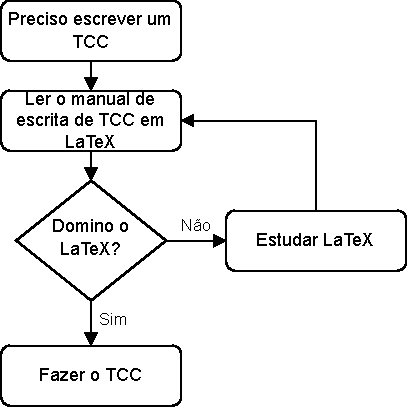
\includegraphics[width=0.5\textwidth]{figuras/diagrama-tcc-latex.pdf}
	\fonte{Elaboração própria.}
\end{figure}

Muitos alunos tem dificuldade em posicionar imagens e tabelas em \LaTeX. O \verb|[h]| no \verb|\begin{figure}[h]| indica que o autor deseja que o \LaTeX\ posicione a imagem tal como está no texto. Substituindo por \verb|[t]| indicamos que desejamos no topo da página, o que geralmente resulta na imagem sendo incluída no topo da próxima página. Por fim, se o \verb|[h]| for insuficiente, use o \verb|[H]| para obrigar o \LaTeX\ a posicionar a imagem tal como no seu código-fonte. Cuidado, isso pode gerar problemas!

Para controlar o tamanho da figura, altere o multiplicador \verb|0.5| no comando \verb|\includegraphics[width=0.5\textwidth]|. Isso controla a largura da imagem. A altura é ajustada com base na largura automaticamente.

Todas as figuras e tabelas devem ter sua breve descrição na parte superior e a indicação de autoria na parte inferior.

\subsubsection{Tabelas}

A criação de tabelas no \LaTeX\ é uma arte. De início, use sites como o \href{https://www.tablesgenerator.com/}{tablesgenerator.com}. Nele você graficamente desenha a tabela que deseja e ele gerará o código \LaTeX. 

% ---
% Conclusão
% ---
\section{Considerações finais}

Elemento obrigatório. A conclusão/considerações finais é a parte final do artigo, na qual se apresentam as conclusões correspondentes aos objetivos e/ou hipóteses. Na conclusão o autor faz um arremate da sua pesquisa, ou de parte dela, retomando o problema. Faz uma análise da pesquisa trazendo resultados obtidos ou dados alcançados, podendo também incluir sugestões.


% ----------------------------------------------------------
% ELEMENTOS PÓS-TEXTUAIS
% ----------------------------------------------------------
\postextual

% ----------------------------------------------------------
% Referências bibliográficas
% ----------------------------------------------------------
\bibliography{referencias}

% ----------------------------------------------------------
% Glossário
% ----------------------------------------------------------
%
% Há diversas soluções prontas para glossário em LaTeX. 
% Consulte o manual do abnTeX2 para obter sugestões.
%
%\glossary

% ----------------------------------------------------------
% Apêndices
% ----------------------------------------------------------

% ---
% Inicia os apêndices
% ---
\begin{apendicesenv}
   \chapter{Exemplo de Apêndice}

   \lipsum[55-56]
\end{apendicesenv}


% ----------------------------------------------------------
% Anexos
% ----------------------------------------------------------
\begin{anexosenv}
   \chapter{Exemplo de Anexo}

   \lipsum[31]
\end{anexosenv}

% ----------------------------------------------------------
% Agradecimentos
% ----------------------------------------------------------

\section*{Agradecimentos}
Texto sucinto aprovado pelo periódico em que será publicado. Último 
elemento pós-textual.

\end{document}